\iffalse
\section{Network Model}\label{model}
\begin{table*}[t]
\setlength{\belowcaptionskip}{0pt}
\normalsize
\caption{Notations}
\label{notation}
\centering
\begin{tabular}{c|c}
\hline
$G\!=\!(V,E)$&Undirected graph with nodes and edges\\
%\hline
%$V$&Set of nodes in the graph\\
%\hline
%$E$&Set of links in the graph\\
%\hline
%$R(v)$&Router-ID of node $v$\\
\hline
$L(u,v)$&Direct link cost between node $u$ and node $v$\\
\hline
$r(u,v)$&The link failure probability between node $u$ and node $v$\\
\hline
 $G'=G^w_{(u,v)}$  &The network topology when the edge
$(l,m)\in E$ change its weight to $w$\\
\hline
$T_c$&Shortest path tree rooted at node $c$\\
\hline
$T_{c}^{G'}$ &Shortest path tree rooted at node $c$ in $G'$ \\
\hline
$C_c(v)$ &The shortest cost from $c$ to $v$ in the original network$G\!=\!(V,E)$\\
\hline
$C_c^{G'}(d)$ &The shortest cost from node $c$  to node $d$ in the network $G'$\\
\hline
$N(v)$&Neighbors of node $v$\\
\hline
$D_c(v)$&Descendants of node $v$ (itself is included) in $T_c$\\
\hline
$D_c^{G'}(v)$&Descendants of node $v$ (itself is included) in $T_{c}^{G'}$\\
\hline
$N_{c}(v)$&Next-hop set computed by node $c$ for destination node $v$\\
\hline
$B_{c}(v)$&Best next-hop computed by node $c$ for destination node $v$\\

%\hline
%$p(v)$&tentative parent of $v$\\
%\hline
%$d(v)$&tentative cost from $c$ to $v$\\
\hline
\end{tabular}
\end{table*}

In this paper, we will limit our research to intra-domain link state routing protocols, e.g. OSPF and IS-IS. Each router in a single routing area maintains an identical network map which allows them to compute the shortest path to every other router in a routing area. Then each router construct its FIB table employing the above information. When a packet arrives at a router, a destination address based method is using to determine how to forward the packets to its corresponding interface. When the network topology changes, the routers adjacent to the changed component detects the change and then propagates the information to its neighboring router through the link state advertisement (LSA) information. After a period of time, all routers in this routing area are aware of  the change information and update their routing tables accordingly, then the network is at a stable state.


In the following sections, a network is modeled as a simple, undirected weighted graph $G=(V,E)$, where $V$ and $E$ respectively denote the set of nodes (routers) and the set of edges (links) in the network. Every link $(u,v)\in E$ in the network has an associated integer weight $L(u,v)$ and a failure probability $r(u,v)$. And the weights of the links in the network are symmetric.
$C_c(v)$ is the lowest cost from $c$ to $v$ in the network.
We use $N(v)$ to denote the neighbor set of the node $v$.
For a node $u\in N(V)$, we have $C_u(v)=C_v(u)=L(u,v)$.

In a link state routing network, the computing node $c$ builds a shortest path tree $T_c$ rooted at itself, containing
all the nodes in the network as potential destinations in the link state routing protocols, such as OSPF and IS-IS.
Then the router $c$ construct its FIB table based on the above information.
In particular, we use $B_{c}(v)$ to represent the best/default candidate,
which lies along the shortest path from $c$ to $v$.
Since $T_c$ is a shortest path tree, leading to the following lemma.
\begin{lemma} {\bf The Best Next-Hop Rule}
\label{bestnh}
\begin{equation}
B_c(v)=\begin{cases}
v&\mbox{$P_c(v)=c$}\\
B_c(P_c(v))&\mbox{$P_c(v)\neq c$}
\end{cases}
\end{equation}
\end{lemma}
Equation (\ref{bestnh}) in Lemma \ref{bestnh} means the best next-hop
$B_c(v)$ for a destination $v$ is $c$'s direct
child along the path from $c$ to $v$ in $T_c$.
A shortest path routing algorithm, such as open shortest path first (OSPF) \cite{moy1998rfc,moy1998ospf},
computes a single next-hop $B_{c}(v)$ by employing equation (\ref{bestnh})
at each step when a new node $v$ is added to the SPT.

We use $G'=(V,E,(l,m,w))$ to represent the new topology when the edge
$(l,m)\in E$ change its weight to $w$, $C_c(v,(l,m,w))$ is the shortest cost from node $c$  to node $v$ in the new network $G'=(V,E,(l,m,w))$.
$T_{c}(c,x,w)$ denote the new shortest path tree when the edge $(c,x)\in T_c$ change its weight to $w$.
For ease of reading, we summarize some  symbols in the Table \ref{notation}.

 $T_{c}$ represent a shortest path tree rooted at $c$, $D(T_{c},v)$ represent the descendants of node $v$ (node $v$ is excluded) in $T_{c}$,
$C_c(v)$ is the shortest cost from node $c$  to node $v$ in the original network $G$.
\fi




\section{Incremental Alternates Computation}\label{iac}
\iffalse
Given sets of nodes $N \in V$, $I(N)=\{S(e)\notin N, E(e) \in N\}$, $O(N)=\{S(e)\in N, E(e) \notin N\}$,
obviously $I(N)=O(N)$ in an undirected connected graph $G$.
\fi

\subsection{Basic Idea}
On a router $c$, we focuses on how to efficiently compute alternate next hops for each destination.
We would like to adopt the criterion of \textbf{LFC}, or \textbf{NPC}, or \textbf{DC},
 in Section \ref{criteria} for different scenarios.
By carefully investigating each criterion, we can see that the difficulty
lies in computing, for each destination $d$, the lowest cost from each neighbor $x$ to $d$ (i.e., $C_{x}(d)$),
with $C_{x}(b)$ just being a special case. All the other costs,
including $C_{c}(d), C_{b}(d)$ and $C_{x}(c)$, are already available
since $c$ always maintains a shortest path tree rooted at itself,
while $C_{b}(d)$ is just $C_{c}(d)-C_{c}(b)$, and $C_{x}(c)$ is just $C_{c}(x)$.

Typical LFA implementations of nowadays router vendors naively maintain a SPT for each neighbor $x$,
thus requires $O(k)$*\textbf{SPT} time and space, where \textbf{SPT} is the complexity of constructing a SPT
from scratch. For nodes with a large number of neighbors, this will become
a bottleneck. TBFH \cite{TBFH} and DMPA \cite{dmpa} accelerate the computation at the cost of
failure repair capability and route availability, since they each utilize a criteria that is more restrict than \textbf{DC}.
For example, DMPA adopts $C_{c}(u)-C_{c}(x)+L(u,d)<C_{c}(d)$, where $u$ is a descendant of $x$,
and the left-hand equation is provably no less than $C_{x}(d)$. Thus DMPA, as well as TBFH,
computes less alternate next hops than our IAC algorithm which strictly follows the criterion of \textbf{DC}.
In addition, DMPA and TBFH cannot be easily adapted to follow \textbf{NPC} while IAC's
unified framework can also handle \textbf{NPC}.



Our algorithm IAC is actually embedded in a dynamic shortest path tree (SPT) algorithm, which takes
a graph and the corresponding SPT as input, and performs incremental shortest path computation
with the sign of some specific link cost simply reversed, i.e., from $\ell$ to $-\ell$. During this specific
dynamic update process, the cost from each neighbor $x$ to each destination $d$ can be efficiently computed,
and the alternates can be computed exactly according to each LFA criterion, achieving high speed, low space and
good quality simultaneously.

\iffalse
Since each node independently computes its next-hops for all destinations,
in the rest of the paper, our algorithm will be
described with respect to a particular node $c$ that performs such
kind of computation.

We denote the cost of the path from $c$ to $v$ in $T_{c}$ by $C_{c}(v)$,
the children of $v$ in $T_c$ by $H_c(v)$,
the parent of $v$ in $T_c$ by $P_{c}(v)$,
and the descendants of $v$ in $T_c$ by $D_c(v)$, with $c$ itself included.
\fi
\iffalse
\begin{figure*}[b]
        \centering
        \begin{subfigure}[b]{0.32\textwidth}
                \centering
                \includegraphics{shortpathtree}
                \caption{$T_{c}$}
              \label{spttree}
        \end{subfigure}
        \begin{subfigure}[b]{0.32\textwidth}
                \centering
                \includegraphics{sachange}
                \caption{$T'_{c}$ when $L(c,a)=0$}
                \label{spttreechange1}
        \end{subfigure}
         \begin{subfigure}[b]{0.32\textwidth}
                \centering
                \includegraphics{sbchange}
                \caption{$T'_{c}$ when $L(c,b)=0$}
                \label{spttreechange2}
        \end{subfigure}
        \caption{An example for explaining some Theorems}
        \label{theoremexample}
\end{figure*}
\fi
%To compute a set $N_{c}(v)$ of next-hops for $v$, we start with
%a simple rule called downstream criterion (DC) \cite{incits8473iso} rule.

\iffalse
\begin{figure}[h]
\centering
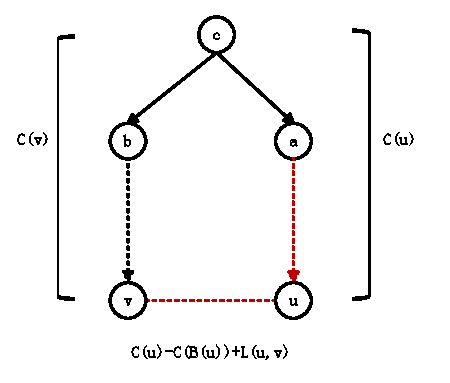
\includegraphics[width=3in]{proof}
\caption{Next-Hop contribution rule illustration}
\label{proofnh}
\end{figure}
\fi
\iffalse
\begin{figure}[t]
\centering
%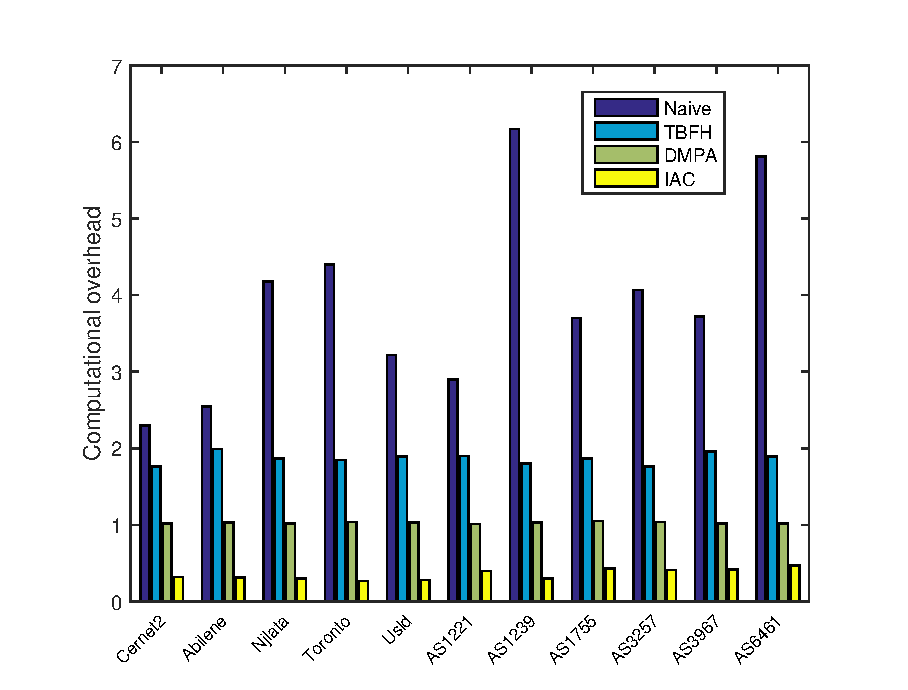
\includegraphics[width=3in]{realcomputationoverhead}
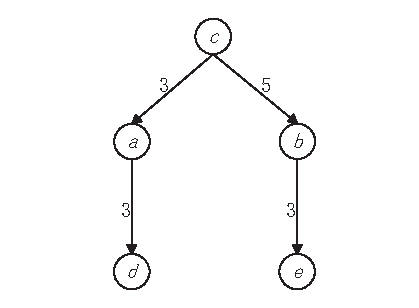
\includegraphics[width=2in]{dcspt}
\caption{Shortest path tree after link change}
\label{ispfspt}
\end{figure}
\begin{figure}[t]
\centering
%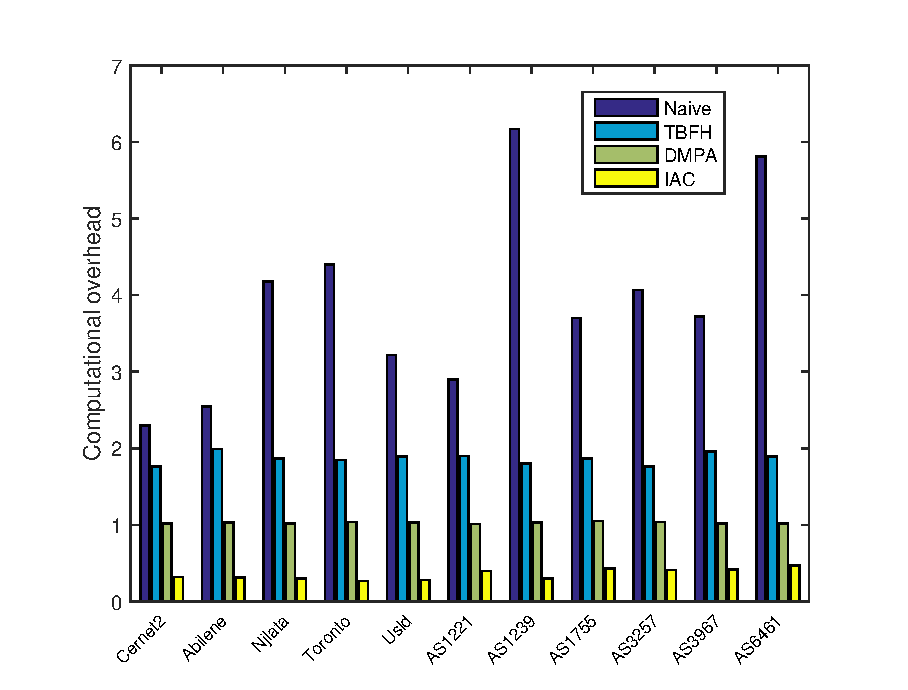
\includegraphics[width=3in]{realcomputationoverhead}
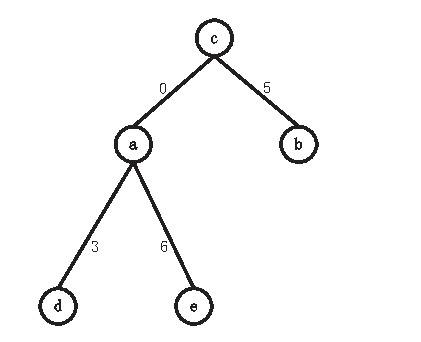
\includegraphics[width=2.5in]{dcsptcha1}
\caption{Shortest path tree after link change}
\label{ispfspt}
\end{figure}
\begin{figure}[t]
\centering
%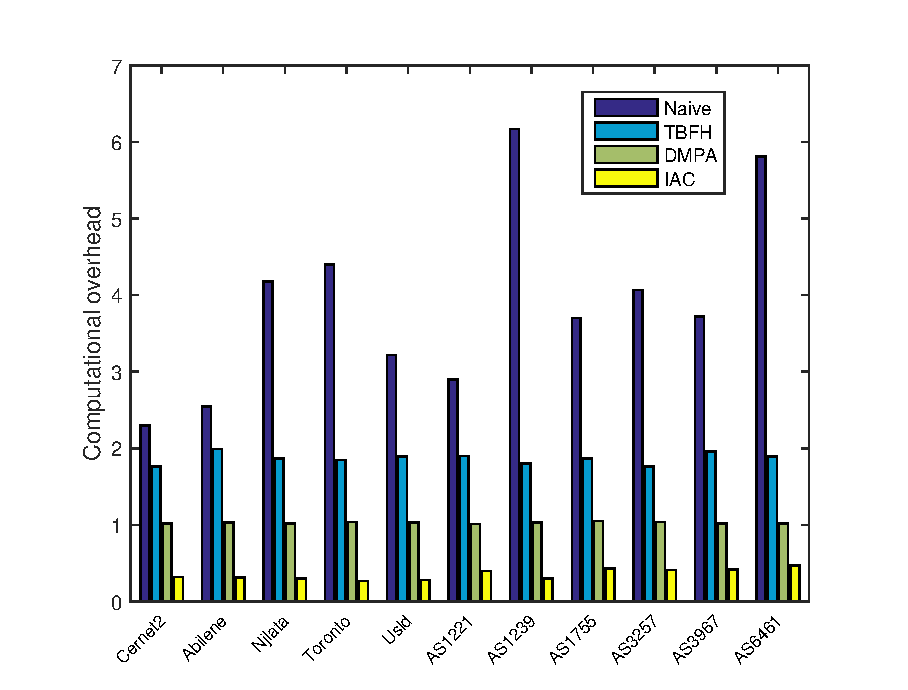
\includegraphics[width=3in]{realcomputationoverhead}
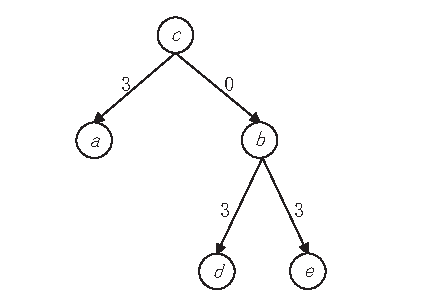
\includegraphics[width=2.5in]{dcsptcha2}
\caption{Shortest path tree after link change}
\label{ispfspt}
\end{figure}
\fi
\iffalse
\begin{theorem}\label{loop-free}
For packets destined to a destination $d$, if any node $c$ ($c \ne d$)
forwards them only to some nodes satisfy $C_v(d)<C_c(d)$,
there will be no loop in the network.
\end{theorem}
\begin{proof}
Consider a forwarding path $<v_{1}, v_{2}, ..., v_{k}, ...>$.
By the DC rule, we have $C_{(v_1)}(d) >C_{(v_2)}(d)$, $C_{(v_2)}(d) >C_{(v_3)}(d), ...$
$C_{(v_k)}(d) >C_{(v_(k+1))}(d)$, and so on. So there exists a strict partial order
between any two nodes on the path, and no node can appear twice on the
path, which means there is no loop.
\end{proof}
\fi
\iffalse
The DC rule is the basis of many loop-free multipath routing algorithms
\cite{Narvaez99efficientalgorithms, Yang_Source:2006, TBFH},
which differ in their ways to find such neighboring nodes that satisfy this rule.
\footnote{Their ways are also the root cause of their high complexity.}
\fi
\iffalse
In order to compute $C_v(d)$, it need to construct multiple
shortest path trees rooted at its neighbors,
so the induced cost will be particularly high for high degree nodes.
Therefore we propose a next-hop contribution rule in Theorem \ref {nhc},
which only need information of the local router.
\fi
\iffalse
If we naively compute $C_x(v)$ on node $c$ by constructing a SPT with $x$ as its root,
we will have to construct a SPT for each neighbor of $c$,
and the cost will be particularly high if the degree of $c$ is high.
The method will involve nontrivial computational overhead.
Such computation can consume a considerable
amount of CPU time, preventing other critical routing functions
from being executed. Thus, it is desirable to achieve this
using as little CPU time as possible.

For the actual deployment on the Internet, a LFA-based scheme should introduce a small additional burden on the current deployed routing protocol. This paper is dedicated to finding an efficient LFA-based scheme which is suitable for deploying on an ISP network. In particular, we focus on the following problem:
\textbf{\emph{Given a computing node $c$ and $T_c$, can we find an efficient LFA-based algorithmic technique and the algorithm conforms to the following two conditions:
(1)The time complexity of the algorithm is less than constructing a shortest path tree.
(2) It can provide the same protection ratio with LFA.
}}

\subsection{Algorithm Specification}
\iffalse
Before diving into the detail of IAC algorithm, we first describe DMPA.
DMPA propose a slightly more strict rule, \textbf{The Next-Hop Contribution Rule}, than the DC rule.

\begin{definition}
\label{selection}
Given any two nodes $u$ and $v$ in the shortest path tree $T_{c}$,
if
\begin{equation}
\label{nhc-eq}
C(u)-C(B(u))+L(u,v)<C(v),
\end{equation}
we say $u$ can contribute (the best next-hop for $u$) to (the next-hop set for) $v$.
\end{definition}



\iffalse
\begin{theorem} {\bf (The Next-Hop Contribution Rule)} \\
\label{nhc}
If $u$ can contribute to $v$, then $C_{B(u)}(v)\!<\!C(v)$,
and $c$ can use $B(u)$, the best next hop for $u$, as a next hop for $v$
without introducing forwarding loops.
%as suggested by the DC rule.
\end{theorem}
\fi
We will use an example to illustrate the Next-Hop contribution rule. In the Fig. \ref{proofnh},
$C(u)$ denote the cost of path $p=(c,a...,u)$ in the $T_c$,
$C(v)$ denote the cost of path $p=(c,b...,v)$ in the $T_c$,
$C(u)-C(B(u))+L(u,v)$ denote the cost of  path
$\lambda(p)\circ (u,v)$, where $\lambda(p)$ denote the subpath of $p$ from its second node to its last node and $\circ$ is the path concatenation operator.
We say $u$ can contribute to $v$
if $C(u)-C(B(u))+L(u,v)<C(v)$ is satisfied. Therefore, node $c$ can use $a$ as a validate next hop to $v$.
\iffalse
The merit of the next-hop contribution rule is that, it is very easy
to check whether inequality (\ref{nhc-eq}) can be satisfied for any two
nodes $u$ and $v$ in the SPT, since all terms in inequality (\ref{nhc-eq})
are known at that time.
So at each step when a new node $v$ is added to the SPT,
we can simply check whether any other node $u$ added earlier can contribute to it,
and add $B(u)$ to $N(v)$ if that is true. Similarly, if $v$ can contribute
to $u$, just add $B(v)$ to $N(u)$. In particular, we only need to do this
test if $u$ and $v$ are neighbors in the network, since otherwise $L(u,v)=\infty$
and (\ref{nhc-eq}) can never be satisfied. With this rule,
we can compute $N(v)$ for any node $v$ in a way faster than other multipath algorithms,
without introducing loops.
\fi
\begin{figure}[h]
\centering
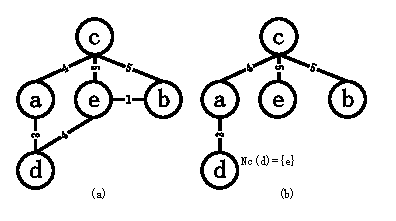
\includegraphics[width=3.8in]{mnpfexample}
\caption{An example for explaining the drawback of DMPA}
\label{drawback}
\end{figure}
Fig. \ref{drawback} gives an example to explain the drawback of DMPA.
Fig. \ref{drawback}(a) is a simple network topology  which consists of
5 node and 6 edges. Fig. \ref{drawback}(b) is a shortest path tree rooted at node $c$. From Fig. \ref{drawback}(b), we can get $C_b(d)=5<C_c(d)=7$, therefore
node $b$ is a feasible backup next-hop from $c$ to $d$. However, we cannot find this feasible backup next-hop employing DMPA. This drawback is due to that node $d$ only considers its neighbors' best next-hop as its potential backup next-hop.
The time complexity of DMPA does not depend on the degree of the calculating router. However, the network availability of DMPA is lower than that of the DC. Unlike the above work, DMPA, however, our main concerns are computational efficiency and network availability, as these are critical for the Algorithm. Based on the existing work on this research area, we for the first time propose an algorithm whose complexity is less than that of Dijkstra's algorithm and without degrading the  network availability of DC.
\label{algorithm}
We first provide two theorems before formally describing the details of the algorithm. The following two theorems describe how to compute all the DC backup next-hop set for node $c$. And the computation overhead can be dramatically reduced via reducing the times of the operation.
\fi


Our main concerns are computational efficiency and network availability, as these are critical for the Algorithm. Based on the existing work on this research area, we for the first time propose an algorithm whose complexity is less than that of Dijkstra's algorithm and without degrading the  network availability of LFA.

For any node $x\in N(c)$, if we can quickly calculate $C_x(v), v\in V$ in the $T_{c}$, then a efficient LFA-based method can be achieved. Therefore, the problem that needs to be solved in this paper can be described as follows: For any node $x\in N(c)$,  if $T_{c}$ it is given, whether could we find an efficient algorithm which can quickly compute $C_x(v), v\in V$ or not. Theorem \ref{computeneighborcost} answers how to solve the above problem and gives proof.



\fi


%\label{algorithm}







\iffalse
\begin{figure}[t]
\centering
\includegraphics[width=3in]{shortpathtree}
\caption{Computation Time for Real and Measured Topologies}
\label{ndavi}
\end{figure}
\begin{figure}[t]
\centering
\includegraphics[width=3in]{sachange}
\caption{Computation Time for Real and Measured Topologies}
\label{ndavi}
\end{figure}
\begin{figure}[t]
\centering
\includegraphics[width=3in]{sbchange}
\caption{Computation Time for Real and Measured Topologies}
\label{ndavi}
\end{figure}
\fi




\iffalse
\begin{figure}[h]
\centering
%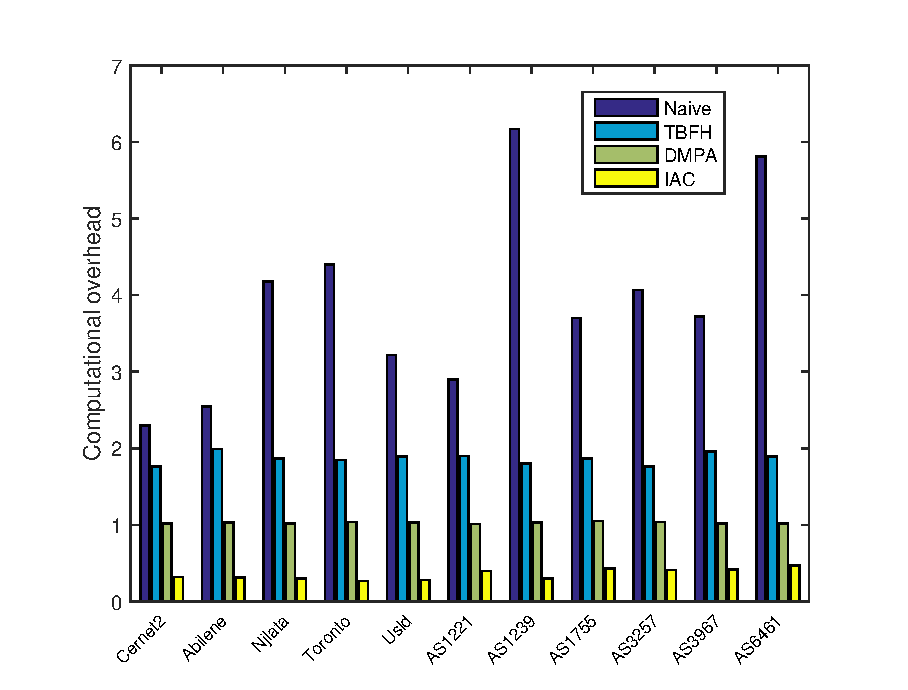
\includegraphics[width=3in]{realcomputationoverhead}
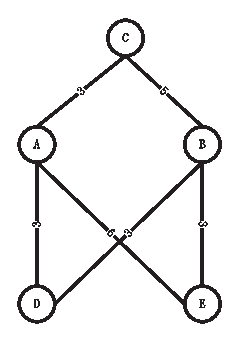
\includegraphics[width=3in]{dcnetworktopology}
\caption{Network topology}
\label{dcnetwork}
\end{figure}
\fi
\iffalse
We will use a simple example to explain the Theorem \ref{dcbackupnexthop}. Fig. \ref{dcnetwork} is a simple network work consists of  5 routers and 6 edges.
Fig. \ref{spttreedc} is a shortest path tree rooted at node $c$, while Fig. \ref{spttreechange1dc} and \ref{spttreechange2dc} respectively represent the new SPT when the weight of the links $(c,a)$  and $(c,b)$  is changed to $0$. Because $e \notin D(T_{c},a)$ and $e \in D(T'_{c},a)$, we can see that node $a$  can be a viable backup next-hop from   $c$ to $e$. Due to $d \notin D(T_{c},b)$, and $d \in D(T'_{c},b)$ ,  node $b$  can be a viable backup next-hop from $c$  to $d$, and also  we can get ode $b$  can be a viable backup next-hop from $c$  to $g$ in the same way.
\fi

\subsection{IAC Algorithm}
\begin{algorithm}[t]
\KwIn{Network graph $G=(V,E)$, the corresponding SPT $T_c$, and the LFA criterion}
\KwOut{$N_c(d)$  ($d \in V \backslash \{c\} $)}
%\SetAlgoNoLine
%\SetAlgoNoEnd
\ForEach{neighbor $x$ of $c$}{
make a temporary copy $T$ of $T_c$\;
\iffalse
\ForEach{$v \in V$}{
 %$v.visited \leftarrow floating$\;
 $C(v) \leftarrow C_c(v)$\;
% $P_{c}^{G_{(c,x)}}(v) \leftarrow P_c(v)$\;
}
\fi
%$c.visited=anchored$\;
 $weight\leftarrow L(c,x) $\;
 $L(c,x)\leftarrow -L(c,x)$\;
 %$newdist\leftarrow C_c(x)+\delta$\;
 %$\delta\leftarrow L(c,x)-weight$\;

 ENQUEUE$(\{x,(c,C_c(x)-2*L(c,x),-2*L(c,x)\})$\;
%\begin{shaded}
%\hl{(In IAC-NA $L(c,x)=-L(c,x)$)}\;
%\end{shaded}


 \iffalse
\For{$m\in D(T_c,x)$}
{
$C'_c(m)\leftarrow C'_c(m)-\delta$\;
%$m.visited=anchored$\;
}
\For{$v \in D(T_c,x)$}{
\For {each neighbor $u$ of $v$}{
\If {$u.visited=floating$ }
{
$newdist \leftarrow C_c(v)+L(v,u)$\;

\If {$newdist <C'_c(u)$}{
$\delta \leftarrow newdist-C'_c(u)$
ENQUEUE$(u,(v,newdist,\delta))$\;}
}
}
}
\fi
\While {$Q$ is not empty}{
$\{m,(p,n,\delta)\}\leftarrow$ EXTRACTMIN(Q)\;
%$P_c^{G_{(c,x)}}(m)\leftarrow n$\;
%$m.visited\leftarrow anchored$\;
adjust $T$ to make $p$ the parent of $m$\;
$C(m)\leftarrow n$\;
\ForEach{descendant $t$ of $m$}{
$C(t) \leftarrow C(t)+\delta$\;
\If{$t\in Q$ and the parent of $t$ in the $Q$ is not equal to its parent in the $T_c$}
{
REMOVE$(n,Q)$\;
}
}
\iffalse\ForEach{$d\in D_c(m)$}
{
$C_{c}^{G_{(c,x)}}(d)\leftarrow C_c(d)+\delta$\;

\If {$d \in D_c(x)$}
{$C_{x}(d)\leftarrow C_{c}(d)-C_{c}(x)$\;
}

\If {$d \notin D_c(x) \land d \in D_c^{G_{(c,x)}}(x)$}
{$C_{x}(d)\leftarrow C_{c}^{G_{(c,x)}}(d)+C_{c}(x)$\;
}
\If {$d \notin D_c(x) \land d \notin D_c^{G_{(c,x)}}(x)$}
{$C_{x}(d)\leftarrow C_{c}(d)+C_c(x)$\;
}

}
\fi
%Compute $C_x(v)$ using Theorem \ref{computeneighborcost}\;
%Add $x$ to $N_c(v)$;\quad\quad\quad\quad\quad\quad\quad\quad\quad\quad\quad\quad\quad\quad\quad\quad\quad\quad\quad
%\hl{(In IAC-NA Compute $C_x(v)$ using Theorem 9)} \;
\ForEach {$t \in D_c(m)$}{
\ForEach {each neighbor $q$ of $t$}{
\If {$C_c(q)>C(m)+L(m,q)$ }
{

$newdist \leftarrow C(m)+L(m,q)$\;
$\delta\leftarrow newdist-C_c(q)$\;
ENQUEUE$(q,(m,newdist,\delta))$\;
}
}
}
}
 $L(c,x)\leftarrow weight$\;
%}
%\ForEach{neighbor $x$ of $c$}
%{
\ForEach{$d \in V\backslash \{c\}$}
{
\If {$d \in D_c(x)$}
{$C_{x}(d)\leftarrow C_{c}(d)-C_{c}(x)$\;
}

\If {$d \notin D_c(x)$ and $d$ is a descendant of $x$ in $T$}
{$C_{x}(d)\leftarrow C(d)+C_{c}(x)$\;
}
\If {$d \notin D_c(x)$ and $d$ is not a descendant of $x$ in $T$}
{$C_{x}(d)\leftarrow C_{c}(d)+C_c(x)$\;
}
\If {the LFA criterion is satisfied}
 {
 add $x$ to $N_c(d)$\;
 }
}
}
\Return $N_c(d) (d \in V \backslash \{c\})$
\caption{Incremental Alternates Computation}
\label{IAC-alg}
\end{algorithm}
\iffalse
\begin{figure*}[t]
\begin{subfigure}[b]{0.20\textwidth}
                \centering
                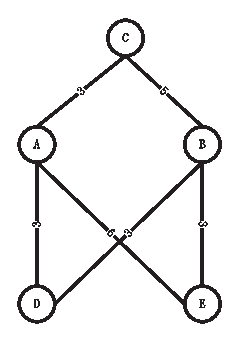
\includegraphics{dcnetworktopology}
                \caption{$T_{c}$}
              \label{dcnetwork}
        \end{subfigure}
        \begin{subfigure}[b]{0.24\textwidth}
                \centering
                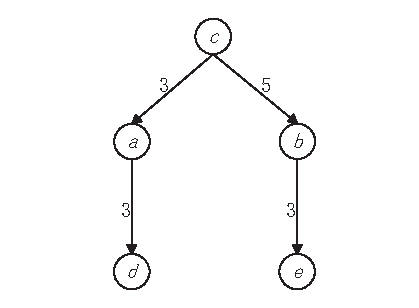
\includegraphics{dcspt}
                \caption{$T_{c}$}
              \label{spttreedc}
        \end{subfigure}
        \begin{subfigure}[b]{0.22\textwidth}
                \centering
                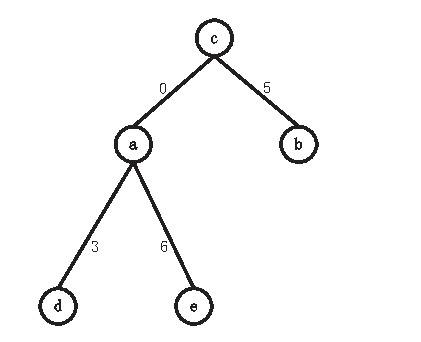
\includegraphics{dcsptcha1}
                \caption{$T_c(c,a,0)$}
                \label{spttreechange1dc}
        \end{subfigure}
         \begin{subfigure}[b]{0.24\textwidth}
                \centering
                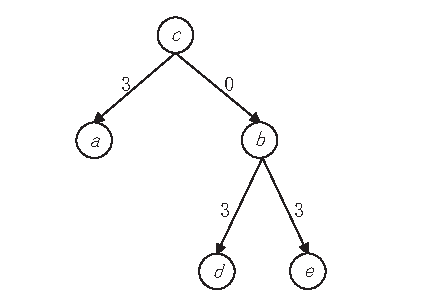
\includegraphics{dcsptcha2}
                \caption{$T_c(c,b,0)$}
                \label{spttreechange2dc}
        \end{subfigure}
        \caption{An example for explaining the Theorem \ref{dcbackupnexthop}}
        \label{theoremdc}
\end{figure*}
\fi

Algorithm \ref{IAC-alg} presents the pseudo code of IAC, where $C_{c}(*)$ and $D_{c}(*)$ denote,
for a give node, the lowest cost from $c$ to it in graph $G$, and its descendants
in the SPT $T_{c}^{G}$ (the superscript $G$ is omitted).
For each neighbor $x$ of $c$, IAC adopts the  ball-and-string model framework\cite{Narv2002New}
to perform an incremental shortest path tree construction for a specific link cost update,
i.e., cost of link $(c,x)$ is changed from $L(c,x)$ to $-L(c,x)$ (line 4).
In the framework, a priority queue $Q$ is maintained to determine the proper node whose
position in the new tree should be fixed.
Each element in $Q$ is of the form ${(u,(p,n,\delta))}$, where $p$ is the potential parent
for node $u$, $n$ denotes the potential lowest cost from $c$ to $u$,
and $\delta$ is the corresponding cost change. The incremental search begins by
inserting element $(x, (c, C_{c}(x)-2*L(c,x), -2*L(c,x)))$ in to the queue (line 5).
Then we extract the node $m$ with the lowest cost in $Q$ and fix its position as well as its descendants' positions, in the new tree (line 7 $\sim$ 8).
For each descendant $t$ of $m$, update the cost from $c$ to
$t$ , and the node $t$ will be removed from the $Q$ if the parent of $t$ in the $Q$ is not equal to its parent in the $T_c$ (line 10 $\sim$ 13).

Note that here we use notation $C(*)$ without any subscript to keep track of the potential
lowest cost from $c$ to a node in the update process.
Then for $m$ and its descendants, we search the potential lower costs of their neighbors,
and insert them into $Q$
if the cost from the root $c$ can be reduced (line 14 $\sim$ 19) to allow further EXTRACTMIN operation.
Note that $m$'s descendants will not be reinserted into $Q$
since their costs and positions are already finalized.
After this incremental tree construction, we compute the cost from $x$ to each node,
and add the node to $N_{c}(d)$ if the LFA criterion is satisfied (line 21 $\sim$ 29).
Finally, after we complete this process for each neighbor of $c$, we return the set of
all alternate next hops for each destination $d$ (line 30) .

\iffalse
For any node $d$ in the network, the corresponding  $C_x(d)$ is computed
for

The $C_x(d)$
While compute the shortest cost $C_x(q)$ when the potential cost of $q$ is smaller than the old value (lines 26).
At last lines 28-31 are using to compute all the LFA next hop set for node $c$.
\fi
%\subsection{Example}


\begin{figure*}[t!]
        \centering
        \begin{subfigure}[b]{0.24\textwidth}
                \centering
                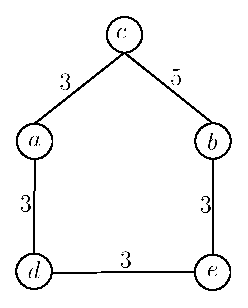
\includegraphics[width=0.8\textwidth]{nettopology}
                \caption{Network $G$}
              \label{spttree21}
        \end{subfigure}
        \begin{subfigure}[b]{0.24\textwidth}
                \centering
                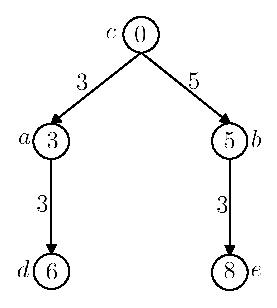
\includegraphics[width=0.8\textwidth]{sptc}
                \caption{$T_{c}$}
                \label{spttreechange22}
        \end{subfigure}
         \begin{subfigure}[b]{0.24\textwidth}
                \centering
                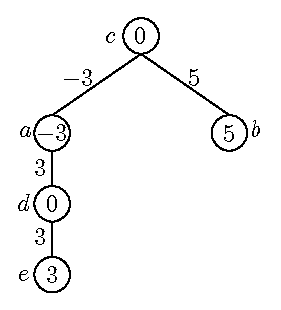
\includegraphics[width=0.8\textwidth]{newsptc}
                \caption{$T_{c}^{G_{(c,a)}}$}
                \label{spttreechange23}
        \end{subfigure}
         \begin{subfigure}[b]{0.24\textwidth}
                \centering
                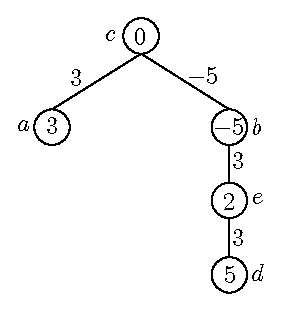
\includegraphics[width=0.8\textwidth]{newsptc1}
                \caption{$T_{c}^{G_{(c,b)}}$}
                \label{spttreechange24}
        \end{subfigure}
        \caption{An example for explaining how ICA works}
        \label{theoremexample}
\end{figure*}


Later, we will prove that this incremental tree construction process actually constructs the SPT for $G_{(c,x)}$, where $G_{(c,x)}$ is the dual graph of $G$ with the sign of $(c,x)$'s cost reversed,
and $C_{x}(d)$ is correctly computed. The proof has to be performed carefully, since the triangle
inequality property may not hold any more in the dual graph with negative link weight.

Before the formal proof, we use the following example to explain how ICA works.
Fig. \ref{spttree21} depicts a network topology consisting of 5 nodes and 6 edges, while the
corresponding SPT $T_{c}$ is depicted in Fig. \ref{spttreechange22}, with $c$ being the root.
For each neighbor or $c$, i.e., $a$ (or $b$), we use Algorithm \ref{IAC-alg} to compute a shortest path tree
$T_{c}^{G_{(c,a)}}$ (or $T_{c}^{G_{(c,b)}}$), where the sign of $(c,a)$'s (or $(c,b)$'s) cost is reversed.
The corresponding SPTs are depicted in Fig. \ref{spttreechange23} and Fig. \ref{spttreechange24}, respectively.

\iffalse
First, the node $a$ is enqueued into the $Q$ with its form \{$(a,(c,-3,-6))$\}.
In the first iteration, $(a,(c,-3,-6))$ will be selected.
The original subtree rooted at $a$  is considered together.
Therefore the node $d$ is selected at the same time.
Since $d$ has an outing edge to $e$, the potential cost and potential cost change of $e$ is calculated, which gives queue \{$(e,(e,3,-5))$\}. Node $d$ is selected in the next iteration.
The new shortest path tree rooted at $c$ is given in the
Fig. \ref{spttreechange23}.
\fi
For the neighbor $a$, according to line 22 $\sim$ 27 in Algorithm \ref{IAC-alg},
we compute the distance from each node to $a$ by:
\begin{align}
&C_a(d)=C_c(d)-C_c(a)=3,  \text{ since } d \in D_c(a) \nonumber\\
&C_a(e)=C(e)+C_c(a)=6,  \text{ since } e \notin D_c(a) \land e \in D_c^{G_{(c,a)}}(a) \nonumber\\
&C_a(b)=C_c(b)+C_c(a)=8,  \text{since } b \notin D_c(a) \land b \notin D_c^{G_{(c,a)}}(a) \nonumber
\end{align}
The correctness of this result, as well as the case for the neighbor $b$,
can be easily verified against the original topology.


\subsection{Theoretical  Analysis}
\iffalse
\begin{definition}
Given a shortest path tree $T_c$ and a network topology  $G'=G_{(c,x)}, (c,x)\in T_c$,
for any node $d\in V, d \neq c, d\in D_c(x)$,
we say the node $d$ change its position in $T_c^{G'}$, if and only if the
$d\in D_c^{G'}(x)$ is satisfied.
\end{definition}
\fi
\iffalse
\begin{theorem}\label{newspt0}
Given a shortest path tree $T_c$,
when the edge $(c,x)\in T_c$ change its weight to 0, the iSPF algorithm can get the correct new SPT $T_c(c,x,0)$.
\end{theorem}
\begin{proof}
The proof for this theorem is exactly the same as that of \cite{Narv2002New}, so the proof is omitted here.
\end{proof}
\begin{definition}
Given a shortest path tree $T_c$, we say a node $d$ change its position in $T_c(c,x,w)$, if and only if the shortest path from $c$ to $d$ is different in the  two trees.
\end{definition}
\begin{theorem}\label{newsptposition0}
Given a shortest path tree $T_c$, for any node $d(d\neq c, d\neq x)$, where $x \in N(c)$
\begin{itemize}
\item[(1)] If the position of the node $d$ in the new SPT $T_c(c,x,0)$ is  changed, then we have  $C_x(d)<C_c(d)$.
 \item[(2)] If $C_x(d)<C_c(d)$ is satisfied,  then the position of the node $d$ in the new SPT $T_c(c,x,0)$ will be changed.
\end{itemize}
\end{theorem}
\begin{proof}
(1)
If the position of the node $d$ in the new SPT $T_c(c,x,0)$ is changed, the node $d$ or its ancestor(s) must be enqueued into the $Q$ using ENQUEUE operation.
Assume that the difference between
the old cost and the potential new cost for the node $d$ is  $\delta$, the new shortest path cost of node $d$ is $C_c(d)-\delta$.
Since only the weight of the link $(c,x)$ is changed to 0, we have $d\in D(T_c(c,x,0),x)$. In $T_c(c,x,0)$, we have $C_c(d,(c,x,0))=C_c(x,(c,x,0))+C_x(d,(c,x,0))$.
Since $C_c(x,(c,x,0))=0$, we have $C_c(d,(c,x,0))=C_x(d,(c,x,0))$.
Because the shortest path from node $x$ to $d$ is not going through node $c$ in $T_c(c,x,0)$, we have $C_x(d,(c,x,0))=C_x(d)$.
Because $C_x(d,(c,x,0))=C_c(d)-\delta$,
we can get $C_x(d)=C_c(d)-\delta$.
Therefore, we have $C_x(d)<C_c(d)$.\\
(2)
Since $C_x(d)<C_c(d)$, the shortest path from node $c$ to node $d$ is not via node $c$.
When the weight of edge $(c,x)$ is changed from $L(c,x)$ to $0$, there exists a path $P=c,x,...,d$ from $c$ to $d$, and the cost of which is $C_c(x)+C_x(d)$.
Because $C_c(x)=0$, the cost of path $P$ is $C_x(d)$.
Therefore, the potential cost change for node $x$ is $C_c(d)-C_x(d)>0$.
The node $x$ will be enqueued into the $Q$ using ENQUEUE operation.
Since only the weight of the link $(c,x)$ is changed to 0, we have $d\in D(T_c(c,x,0),x)$. Therefore, the position of the node $d$ in the new SPT $T_c(c,x,0)$ will be changed.
\end{proof}
\fi
\iffalse
\begin{theorem}\label{newspttree0}
Given a $T_{c}$, $x \in N(c)$, for any node $d(d\neq c, d\neq x)$,
if the
\begin{itemize}
\item[(1)] if $d \notin D(T_{c},x)$ and $C_x(d)<C_c(d)$, then we have  $d\in D(T_c(c,x,0),x)$.
\item[(2)] if $d \notin D(T_{c},x)$ and $d \notin D(T_c(c,x,0),x)$, then we have $C_x(d)<C_c(d)$.
\end{itemize}
\end{theorem}
\begin{proof}

\end{proof}








We have already known that Dijkstra's algorithm \cite{Dijkstra1959A} is not applicable with the networks whose link have negative weights. From the above example, when the link $(c,a)$ change its weight to $-L(c,a)$, the correct new shortest path tree can be constructed using iSPF. Theorem \ref{newspt} indicates that this is not a special case.
\fi
In this section, we use the abbreviated notation $G'$ to represent the dual graph $G_{(c,x)}$ of $G$,
where the link cost of $(c,x)$ changes from $L(c,x)$ to $-L(c,x)$.
\begin{theorem}\label{newspt}
For each neighbor $x$ of node $c$, the dual graph $G'$ contains no negative cycle,
and Algorithm \ref{IAC-alg} constructs the corresponding SPT $T_{c}^{G'}$
and the lowest distance from $c$ to each node.
\end{theorem}
\begin{proof}
%the weight of the link $(c,x)$ is changed to $-L(c,x)$,
We prove by contradiction. Assume there exists a negative cycle in $G'=G_{(c,x)}$, then the cycle must go through $(c,x)$ since
it is the only link with negative cost, i.e., $-L(c,x)$ where $L(c,x)$ is the link cost in the prime graph $G$.
Let the cycle be $(c,x,y,...,c)$, and the lengths of the two paths
$(c,x)$ and $(x,y,...,c)$ in this cycle be $-L(c,x)$ and $Length(x,y,...,c)$ respectively,
then $-L(c,x)+Length(x,y,...,c)<0$. That means $Length(x,y,...,c)<L(c,x)$, which contradicts with our triangle inequality
assumption in $G$ that $L(c,x)$ is the lowest cost between $c$ and $x$.
Therefore, there must exist a SPT in $G'$, and the correctness of the tree construction procedure
in IAC can be proven by following the proof of the ball-and-string algorithm,
since IAC is just a special case with specifically crafted link cost decrease in their incremental
shortest tree algorithm\cite{Narv2002New}.
\iffalse
We will use inductive reasoning to prove this theorem.\\
(1)We first prove
the base case. When the weight of edge $(c,x)$ is changed from $L(c,x)$ to $-L(c,x)$.
The potential parent for node $x$ is $c$, the potential cost for node $x$ is $-L(c,x)$, the potential cost change for node $x$ is $-2*L(c,x)$. The node $x$ will be enqueued into the $Q$ using ENQUEUE operation. After this operation, the queue has one element in the form of
$(x,(c,-L(c,x),-2*L(c,x)))$. Because there is no node can decrease its cost by more than $-2*L(c,x)$. Therefore, all of the descendants of node $x$ will be  placed in the correct positions during the first iteration.\\
(2)The inductive step is the same as in the \cite{Narv2002New}, so we omitted the content.\fi
\end{proof}

\begin{theorem}\label{newsptd}
For $c$'s neighbor $x$ and any node $d$ that is $x$'s descendant in $T_c$,
$C_x(d)=C_c(d)-C_c(x)$.
\end{theorem}
\begin{proof}
Since the path from $x$ to $d$ in the SPT $T_c$ is also the shortest path from $x$ to $d$ in $G$,
$C_c(d)=C_c(x)+C_x(d)$. So we get $C_x(d)=C_c(d)-C_c(x)$.
\end{proof}

\begin{theorem}\label{newsptx}
For $c$'s neighbor $x$ and any node $d$ (other than $c$ and $x$) that is not $x$'s descendant in $T_c$, if
$d$ becomes $x$'s descendant in $T_{c}^{G'}$, then $C_x(d)=C_c^{G'}(d)+C_c(x)$. %$C_c^{G'}(d)=C_c^{G'}(x)+C_x(d)$.
\end{theorem}
\begin{proof}
Let $P$ denote the path from $x$ to $d$ in $T_{c}^{G'}$,
and let  $Length(P)$ denote the cost of $P$.
Let $Q$ denote the shortest path from $x$ to $d$ in $G$, and its cost is $C_x(d)$.
It is obvious that $Length(P) \ge C_{x}(d)$ since $P$ is also a path in $G$.
As $d$ is $x$'s descendant in SPT $T_c^{G'}$,
we know $(c,x) \notin P$, and  $C_c^{G'}(d)=C_c^{G'}(x)+Length(P)$.
Therefore $C_c^{G'}(d) \ge C_c^{G'}(x)+C_x(d)$.

Suppose $Q$ does not pass through $c$,
then we get a non-cycling path $(c,x) \oplus Q$ from $c$ to $d$ in $G'$,
whose path cost will be $C_c^{G'}(x)+C_x(d)$.
Since $C_c^{G'}(d)$ is the lowest cost from $c$ to $d$ in $G'$,
it cannot be larger than $C_c^{G'}(x)+C_x(d)$. Therefore, $C_c^{G'}(d)=C_c^{G'}(x)+C_x(d)$.

Suppose $Q$ passes through $c$,
then $C_x(d)=C_x(c)+C_c(d)$, therefore we get
$C_c^{G'}(d) \ge C_c^{G'}(x)+C_{x}(d) = C_c^{G'}(x)+C_x(c)+C_c(d)=-L(c,x)+L(c,x)+C_{c}(d)=C_{c}(d)$.
As $C_c^{G'}(d)$ can be no larger than $C_{c}(d)$, equality has to be achieved in the last inequation,
which means $C_c^{G'}(d)=C_c^{G'}(x)+C_x(d)$.
%and $Length(P)=C_{x}(d)$

As $C_c^{G'}(x)=-C_c(,x)$, we get $C_x(d)=C_c^{G'}(d)+C_c(x)$ in both conditions.
\end{proof}
\begin{theorem}\label{newsptposition}
For $c$'s neighbor $x$ and any node $d$ (other than $c$ and $x$) that is not $x$'s descendant in $T_c$,
$d$ becomes $x$'s descendant in $T_{c}^{G'}$ if and only if $C_x(d)<C_x(c)+C_c(d)$.
\end{theorem}
\begin{proof}
We first prove if $C_x(d)<C_x(c)+C_c(d)$, then  $d\in D_c^{G'}(x)$.
Since $C_x(d)<C_x(c)+C_c(d)$, the shortest path in $G$ from node $x$ to node $d$
does not pass through node $c$.
Let the path be denoted by $P(x,d)$, then we can construct a non-cycling path
$P(c,d)=(c,x) \oplus P(x,d)$ from $c$ to $d$ in $G_{(c,x)}$,
where $\oplus$ means the concatenation of two paths.
Since the link cost of $(c,x)$ in $G_{(c,x)}$ is $-L(c,x)$,
the cost of $P(c,d)$ in $G_{(c,x)}$ will be $-L(c,x)+C_x(d)$.
On the other hand, from the condition $C_x(d)<C_x(c)+C_c(d)$ we get $C_{x}(d)<L(c,x)+C_{c}(d)$,
which means $C_{c}(d)>-L(c,x)+C_{x}(d)$. Since $d$ is not a descendant of $x$ in $T_{c}$
(i.e., $d \notin D_c(x)$),
at some time, the condition of line 16 in Algorithm \ref{IAC-alg}
will be triggered, and $d$ will be inserted into $Q$ by the ENQUEUE operation in line 19,
and later positioned in the subtree rooted at $x$ as $x$'s descendant (i.e., $d \in D_c^{G'}(x)$).
From Theorem \ref{newspt}, we know the subtree is part of $T_{c}^{G_{(c,x)}}$.

We then prove if $d\in D_c^{G'}(x)$, then  $C_x(d)<C_x(c)+C_c(d)$.
According to Theorem \ref{newsptx}, we know $C_x(d)=C_c^{G'}(d)+L(c,x)$.
%Assume that the potential cost change for node $d$ is  $\delta$, the potential cost of node $d$ is $C_c(d)+\delta$.
%In $T_c^{G(c,x)}$, we have $C_c^{G(c,x)}(d)=C_c^{G(c,x)}(x)+C_x(d)$ according to Theorem \ref{newsptx}.
Since $d \notin D_c(x)$ and $d\in D_c^{G(c,x)}(x)$,
node $d$ must be inserted into the $Q$ by the ENQUEUE operation at some time,
while the cost $C_c^{G'}(d)$ must be less than $C_{c}(d)$ (line 16 in Algorithm \ref{IAC-alg}).
Thus $C_x(d)=C_c^{G'}(d)+L(c,x) < C_c(d)+L(c,x) = C_x(c)+C_c(d)$.
\end{proof}

\iffalse
Since , the shortest path from node $c$ to node $d$ is not via node $c$.
When the weight of edge $(c,x)$ is changed from $L(c,x)$ to $-L(c,x)$,
the potential cost change for node $d$ is $C_c(d)-C_x(d)+C_x(c)>0$.
The node $x$ will be enqueued into the $Q$ using ENQUEUE operation.
Since only the weight of the link $(c,x)$ is changed to $-L(c,x)$, we have $d\in D_c^{G'}(x)$.
\fi








\iffalse
\begin{theorem}
Given a $T_{c}$, $x \in N(c)$, for any node $d(d\neq c, d\neq x)$
\begin{itemize}
\item[(1)] if $v \notin D(T_{c},x)$ and $C_x(v)<C_c(v)+C_x(c)$, then we have  $v\in D(T_c(c,x,-L(c,x)),x)$.
\item[(2)] if $v \notin D(T_{c},x)$ and $C_x(v)=C_c(v)+C_x(c)$, then we have  $v\notin D(T_c(c,x,-L(c,x)),x)$.
\end{itemize}
\end{theorem}

\begin{theorem}\label{newsptposition1}
Given a $T_{c}$, $x \in N(c)$, for any node $d(d\neq c, d\neq x)$
\begin{itemize}
\item[(1)] If the position of the node $d$ in the new SPT $T_c(c,x,0)$ is  changed, then we have  $C_x(d)<C_c(d)+C_x(c)$.
\item[(2)] if $C_x(d)<C_c(d)+C_x(c)$ is satisfied,  then the position of the node $d$ in the new SPT $T_c(c,x,-L(c,x))$ is  changed.
\end{itemize}
\end{theorem}
\begin{proof}
\end{proof}
\begin{theorem}\label{newspttree1}
Given a $T_{c}$, $x \in N(c)$, for any node $v(v\neq c, v\neq x)$
\begin{itemize}
\item[(1)] if $v \notin D(T_{c},x)$ and $C_x(v)<C_c(v)+C_x(v)$, then we have  $v\in D(T_c(c,x,-L(c,x)),x)$.
\item[(2)] if $v \notin D(T_{c},x)$ and $v \notin D(T_c(c,x,-L(c,x)),x)$, then we have $C_x(v)<C_c(v)+C_x(v)$.
\end{itemize}
\end{theorem}
\begin{proof}
\end{proof}
\begin{lemma}\label{nochange}
For any node $m$ in the $G$, if $C_x(v)=C_c(v)+C_x(c)\geq C_c(m)$, the position of the node $m$ will be not changed in the new SPT $T_c(c,x,-L(c,x))$.
\end{lemma}
\begin{proof}
From theorem \ref{newspt}, we can easily get this lemma. Because $C_x(v)= C_c(v)+C_x(c)= C_c(m)$, the node $x$ will not be enqueued into the Queue.
\end{proof}
\begin{theorem}\label{newspttree}
Given a $T_{c}$, $x \in N(c)$, for any node $v(v\neq c, v\neq x)$
\begin{itemize}
\item[(1)] if $v \notin D(T_{c},x)$ and $C_x(v)<C_c(v)+C_x(c)$, then we have  $v\in D(T_c(c,x,-L(c,x)),x)$.
\item[(2)] if $v \notin D(T_{c},x)$ and $C_x(v)=C_c(v)+C_x(c)$, then we have  $v\notin D(T_c(c,x,-L(c,x)),x)$.
\end{itemize}
\end{theorem}
\begin{proof}
(1)We will prove the first part of this theorem  by contradiction. If  $v\notin D(T_c(c,x,-L(c,x)),x)$, from Lemma \ref{nochange} we have $C_x(v)\geq C_c(v)+C_x(c)$. This contradict the $C_x(v)<C_c(v)+C_x(c)$.\\
(2)From Lemma \ref{nochange} we can get the second part of this theorem is correct.
\end{proof}
\fi
%$v\in D(T_c(c,x,-L(c,x)),B_c(v))$,
\iffalse
From Theorem \ref{newsptposition}, we can see that if the shortest path from neighboring node $x$ to $d$ is not going through node $c$.
The node $d$  must be the descendant of node $x$ in the new shortest path tree when the  weight of $(c,x)$ is changed to $-L(c,x)$.
Contrarily, if the node $c$ is included in the shortest path from neighboring node $x$ to $d$. The node $d$  must not be the descendant of node $x$ in the new shortest path tree when the  weight of $(c,x)$ is changed to $-L(c,x)$.
\fi
\begin{theorem}\label{fan}
For $c$'s neighbor $x$ and any node $d$ (other than $c$ and $x$) that is not $x$'s descendant in $T_c$,
$d$ does not become $x$'s descendant in $T_{c}^{G'}$, then $C_x(d)=C_c(d)+C_c(x)$.
\end{theorem}
\begin{proof}
From Theorem \ref{newsptposition}, since $d \notin D_c(x)$ and $d \notin D_{c}^{G'}(x)$,
we have $C_x(d) \ge C_x(c)+C_c(d)$.
On the other hand, since $C_x(d)$ is the lowest cost from $x$ to $d$ in $G$,
$C_x(d) \le C_x(c)+C_c(d)$.
Combining these two inequalities, we get $C_x(d)=C_x(c)+C_c(d)=C_c(d)+C_c(x)$.
%Therefore, the lemma can be easily verified.
\end{proof}


\iffalse
\begin{theorem}\label{computeneighborcost}
Given a shortest path tree $T_c$ and a network topology  $G'=G_{(c,x)}, (c,x)\in T_c$, for any node $d (d\neq c \land d\neq x)$
\begin{itemize}
\item[(1)] if $d \in D_c(x)$, then we have $C_{x}(d)=C_{c}(d)-C_{c}(x)$.
\item[(2)] if $d \notin D_c(x)$ and $d \in D_c^{G'}(x)$, then we have
 $C_{x}(d)=C_{c}^{G'}(d)+C_{c}(x)$.
\item[(3)] if $d \notin D_c(x)$ and $d \notin D_c^{G'}(x)$, then we have
 $C_{x}(d)=C_{c}(d)+C_c(x)$.
\end{itemize}
\end{theorem}
\begin{proof}
(1) Since $d \in D_c(x)$, we have $C_{c}(d)=C_{c}(x)+C_{x}(d)$. Therefore, we can easy get $C_{x}(d)=C_{c}(d)-C_{c}(x)$.

(2) According to Theorem \ref{newsptx}, we have $C_{c}^{G'}(d)=C_{c}^{G'}(x)+C_{x}(d)$ if  $d \in D_c^{G'}(x)$.
Because $C_{c}^{G'}(x)=-C_c(x)$, we have
$C_{x}(d)=C_{c}^{G'}(d)+C_c(x)$.

(3) From lemma \ref{fan}, we have $C_{x}(d)=C_{c}(d)+C_c(x)$.
\end{proof}
\fi

\iffalse
\begin{theorem}\label{dcextend}
Given a computing node $c$ and $T_{c}$, for any node $x \in N(c)$ , $T'(c)$ is the new shortest path tree rooted at node $c$  when the weight of link $(c,x)$ is changed to 0. For any node $v(v\neq c, v\neq x)$, if $v \notin D(T_{c},x)$ and $v \in D(T'_{c},x)$, then we can get $C_{x}(v)<C_{c}(v)$.
\end{theorem}
\begin{proof}
Assuming that  $B_{c}(v)=y, y\neq x$ in the $T_{c}$, we have $C_{c}(v)=C_{c}(y)+C_{y}(v)$.
Since $v \in D(T'_{c},x)$, we can obtain $C'_{c}(v)=C_{c}(x)+C_{x}(v)$, where  $C'_{c}(v)$ is the cost from node $c$ to node $v$ in the $T'_{c}$. Because the weight of link $(c,x)$ in the $T'_{c}$ is 0, we can get  $C'_{c}(v)=C_{x}(v)$(1). According to that $v \notin D(T_{c},x)$ and $v \in D(T'_{c},x)$ , we can obtain $C'_{c}(v)<C_{c}(v)$  (2). Combining the equation (1) with (2), we have $C_{x}(v)<C_{c}(v)$.
\end{proof}
\fi
\iffalse
\begin{theorem}\label{dcbackupnexthop}
Given a shortest path tree $T_c$, for any node $d(d\neq c, d\neq x)$, if $d \notin D(T_{c},x)$ and $v \in D(T_{c}(c,x,0),x)$, then we can get $N_c(d)=N_c(d)\cup {x}$.
\end{theorem}
\begin{proof}
From the Theorem \ref{newspt0}, Theorem \ref{newsptposition0} and DC rule, we can see that the node   $x$ is a viable backup next-hop from node $c$ to node $d$, therefore we have $N_c(d)=N_c(d)\cup {x}$.
\end{proof}

\begin{theorem}\label{algorithmcorrect}
Given a shortest path tree $T_c$ and a network topology  $G'=G_{(c,x)}, (c,x)\in T_c$, the value of $C_x(d), d\neq c \land d\neq x$ can be correctly computed by IAC.
\end{theorem}
\begin{proof}
For any node $d\in T_c^{G'}$, the calculation of the value of $C_x(d)$ can be divided into three cases.

(1) If $d \in D_c(x)$, the lines 24-25 are executed.

(2)If $d \notin D_c(x) \land d \notin D_c^{G'}$, the lines 26-27 are executed.

(3)If $d \notin D_c(x) \land d \notin D_c^{G'}$, the lines 28-29 are executed.

According to Theorem \ref{computeneighborcost}, all of the $C_x(d), d \in V$ will be calculated when the lines ($23 \sim 29$) of the IAC are executed.
\end{proof}

\begin{theorem}\label{fullprooof}
Algorithm IAC can compute all the next hop set for node $c$ that satisfies the LFA Rule.
\end{theorem}
\begin{proof}
From Theorem \ref{algorithmcorrect}, all of the $C_x(d), d \in V$ will be calculated when the lines ($23 \sim 29$) of the IAC are executed.
As long as we know the above values, we can use the LFA rule to compute all the LFA next hop set for node $c$ (lines $30 \sim 31$).
\end{proof}
\fi



\iffalse
Now we will show the performance of the algorithm, including the time complexity and the number of backup next-hop computed by LFA. From theorem \ref{iaccomplexity}, we can see that the computational complexity of IAC is less than that of constructing a shortest path tree. From theorem \ref{fullprooof}, we can see that the IAC can compute all the backup next-hop set which satisfies the LFA Rule. We will describe the Theorem \ref{iaccomplexity} and Theorem \ref{fullprooof} in detail, and also their correctness is proved.
\fi

Incrementally constructing the SPT for the dual graph $G'$
and efficiently computing $C_x(d)$  for each $x$ and $d$ are
critical to IAC's correctness, completeness and efficiency.
Theorem \ref{newsptd}, Theorem \ref{newsptx} and Theorem \ref{fan} show concrete support
for line 22 $\sim$ 27 in Algorithm \ref{IAC-alg},
where $C_x(d)$ is computed in different ways for each situation.
%Next, we provide a simple analysis on IAC's complexity.

%\begin{theorem}\label{iaccomplexity}
%The computational complexity of IAC is less than $\lg|V|\sum_{i=1}^k{M_{i}}$ when the queue is implemented as a binary heap.
%\end{theorem}
%\begin{proof}
To compute all the backup next-hop sets on node $c$ for each destination in the network,
IAC needs to run the incremental SPT construction (i.e., iSPF) algorithm $k$ times,
where $k$ is the number of its neighbors.
For one neighbor $x$, let $\delta_{n}$ denote the number of potentially affected nodes,
and $\delta_{e}$  the number of edges attached to any of these nodes.
According to the ball-and-string model\cite{Narv2002New},
the worst case complexity of the iSPF procedure for this neighbor will be
$O(\delta_{e}*lg(\delta_{n}))$ with a binary heap, or $O(\delta_{e}+\delta_{n}*lg(\delta_{n}))$ with a Fibonacci heap.
The remaining part, including duplicating the tree and
computing $C_{x}(d)$ for all destinations, requires only $O(|E|+|V|)$ time.
So the worst case complexity of IAC will be no more than $O(k*|V|*lg|V|)$ (or $O(k*|E|*lg|V|)$,
depending on the heap implementation). However, in practice, we find this bound to be
quite loose, and IAC is always faster than computing a single SPT.
This may be due to the special link cost decrement operation in IAC,
and we leave why this happens to future studies.

\iffalse
Therefore, the computational complexity of the Algorithm IAC is $\sum_{i=1}^k{M_{i}*lgN_{i}}.  \leq \lg|V|\sum_{i=1}^k{M_{i}}$.
Since $N_{i}<|V|$, the computational complexity of IAC is less than $\lg|V|\sum_{i=1}^k{M_{i}}$.
\fi
%The computational complexity in IAC for this neighbor $i$ can be expressed as $O(M_{i}lgN_{i})$ according to \ref{Narv2002New}.
%\end{proof}

\iffalse
\begin{theorem}\label{iacfullprooof}
Algorithm IAC can compute all the backup next-hop set that satisfies the LFA Rule.
\end{theorem}
\begin{proof}
We will prove the theorem by contradiction. Supposing that there is a node $d(d\neq c, d\neq x)$, $d \notin D(T_{c},x)$ and $C_x(d)<C_{c}(d)$, when the IAC is terminated. For any node $x \in N(c)$,
if $C_x(d)<C_{c}(d)$, we have $d \in D(T_{c},x)$ according to Theorem \ref{newspt0} and
Theorem \ref{newsptposition0}. This contradicts the assumption.
\end{proof}
\fi
\iffalse
\subsection{Discussions}
IAC algorithm can only handle DC rule. However, it cannot be directly applied to LFC and NPC rules. Therefore, IAC cannot completely solve LFA problem.
We want to ask whether we can find an general algorithm that can completely and efficiently solve LFA. We will discuss this issue in the following sections.
\fi
\iffalse
\subsection{Discussions}
In the following, we will discuss how to apply the INC algorithm to compute all the backup next-hop set which meets the LFC rule. The LFC can be expressed as follows:

For packets destined to a destination $v$, node $c$ ($c \ne v$)
can forward them to its neighboring node $x$ if
\begin{equation}\label{eqn-LFC}
C_x(v)<C_c(v)+C_c(x).
\end{equation}
The resulting paths are loop-free and will reach the destination.

The following two theorems describe how to compute all the LFC backup next-hop set for node $c$. And the computation overhead can be dramatically reduced via reducing the times of the operation.

\begin{theorem}\label{lfcextend}
Given a computing node $c$ and $T_{c}$, for any node $x \in N(c)$ , $T'(c)$ is the new shortest path tree rooted at node $c$  when the weight of link $(c,x)$ is changed to $-L(c,x)$. For any node $v(v\neq c, v\neq x)$, if $v \notin D(T_{c},x)$ and $v \in D(T'_{c},x)$, then we can get $C_{x}(v)<C_{c}(v)+C_{c}(x)$.
\end{theorem}
\begin{proof}
Assuming that  $B_{c}(v)=y, y\neq x$ in the $T_{c}$, we have $C_{c}(v)=C_{c}(y)+C_{y}(v)$.
Since $v \in D(T'_{c},x)$, we can obtain $C'_{c}(v)=C_{c}(x)+C_{x}(v)$, where  $C'_{c}(v)$ is the cost from node $c$ to node $v$ in the $T'_{c}$. Because the weight of link $(c,x)$ in the $T'_{c}$ is $-L(c,x)$, we can get  $C'_{c}(v)=C_{x}(v)-L(c,x)$(1). According to that $v \notin D(T_{c},x)$ and $v \in D(T'_{c},x)$ , we can obtain $C'_{c}(v)<C_{c}(v)$  (2). Combining the equation (1) with (2), we have $C_{x}(v)<C_{c}(v)+L(c,x)$. Because $C_{c}(x)=L(c,x)$, we can get $C_{x}(v)<C_{c}(v)+C_{c}(x)$.
\end{proof}
\begin{theorem}\label{lfcbackupnexthop}
Given a computing node $c$ and $T_{c}$, for any node $x \in N(c)$ , $T'(c)$ is the new shortest path tree rooted at node $c$  when the weight of link $(c,x)$ is changed to 0. For any node $v(v\neq c, v\neq x)$, if $v \notin D(T_{c},x)$ and $v \in D(T'_{c},x)$, then we can get $N_c(v)=N_c(v)\cup {x}$.
\end{theorem}
\begin{proof}
From the  Theorem \ref{lfcextend}
and LFC rule, we can see that the node   $x$ is a viable backup next-hop from node $c$ to node $v$, therefore we have $N_c(v)=N_c(v)\cup {x}$.
\end{proof}
In order to implement LFC, we only need to change the line 3 of the INC as  $L(c,x)\leftarrow -L(c,x)$. From Theorem \ref{mpnedccomplexity} and Theorem \ref{fulldcprooof}, we can also get the same conclusion that the computation complexity our algorithm is less than constructing a shortest path tree and can provide the same network availability with DC. Since the proofs of Theorem \ref{mpnedccomplexity} and \ref{fulldcprooof}  are similar
to those of \ref{mpnecomplexity} and \ref{fullprooof}, so we omitted them.
\begin{theorem}\label{mpnedccomplexity}
The computational complexity of INC is less than $O(|E|lg|V|)$ ��
\end{theorem}

\begin{theorem}\label{fulldcprooof}
Algorithm INC can compute all the backup next-hop set that satisfies the LFC Rule.
\end{theorem}

\fi












\iffalse

Since $N_n = |V|$ and $N_e = |E|$, Algorithm \ref{dijk}
costs at most $O(|V|)+O(N_{n}*\lg(N_{n})+N_{e}) = O(|V|*\lg(|V|)+|E|)$,
which is similar to the complexity of a full shortest path computation.



where $em_Q$ and $dk_Q$ are times needed to perform extract minimum and decrease key
operations in the $Q$, respectively.
Since there are at most $V$ nodes in the queue,
$T_e=O(1), T_{x}=\lg(N_n)$ and $T_{k}=O(1)$ when the queue is implemented as a Fibonacci heap \cite{knuth1977generalization},
and the total time is at most $O(N_n*\lg(N_{n})+N_e)$.

Since $N_n = |V|$ and $N_e = |E|$, Algorithm \ref{dijk}
costs at most $O(|V|)+O(N_{n}*\lg(N_{n})+N_{e}) = O(|V|*\lg(|V|)+|E|)$,
which is similar to the complexity of a full shortest path computation.


Because there are at most $|V|$ nodes in the $Q$,
a node is extracted from $Q$ and an edge is performed decrease key
takes $O(lg|V|)$ and $O(1)$ time complexity respectively
on Fibonacci heap \cite{knuth1977generalization}.

When a node is extracted from the queue, whose neighbors will be visited.
The unvisited neighbors have an \emph{Enqueue} operation, while the visited
neighbors and the node itself may have an \emph{Add} operation.
However, both of the functions have constant complexity.
Therefore, the complexity of Algorithm \ref{DMPA} is in $O(|V|lg|V|+|E|)$.


In this section, we will explain the time complexity of MPA in detail.
In order to maintain nodes, which need to be updated the positions (parents) and costs, we adopt a priority queue.
We define $N_{n}$ is the node number which must change their cost or parent attributes (or both),
and $N_{e}$ is the edge number that may cause any node in
the queue to change its cost (This is implemented by the decrease-key operation of the priority queue).
Assume the time needed by ENQUEUE to enqueue a node is $T_e$, the time
by EXTRACTMIN to extract the node with the minimum cost is $T_{x}$,
and the time by ENQUEUE (decrease-key) to update a node existing in the queue is $T_{k}$.
Since each of the $N_{n}$ nodes has to be enqueued and extracted exactly once,
and each of the $N_e$ edges can cause at most one decrease-key operation, the total queue operation time in all
execution of Algorithm \ref{dijk} is at most $O(N_{n}*T_{e}+N_{n}*T_{x}+N_{e}*T_{k})$.
Beside queue manipulations, some operations are called at most two times for each of the $N_e$ edges,
including modifying the next-hop sets,
while others are called at most once for each of the $N_n$ nodes to set their attributes.
Each of them can be completed in constant time (or constant amortized time), and  they cost $O(N_n+N_e)$ in total.
So the final time for all execution of Algorithm\ref{dijk} is still $O(N_{n}*T_{e}+N_{n}*T_{x}+N_{e}*T_{k})$.

Since there are at most $N_n$ nodes in the queue,
$T_e=O(1), T_{x}=\lg(N_n)$ and $T_{k}=O(1)$ when the queue is implemented as a Fibonacci heap \cite{knuth1977generalization},
and the total time is at most $O(N_n*\lg(N_{n})+N_e)$.

Since $N_n = |V|$ and $N_e = |E|$, Algorithm \ref{dijk}
costs at most $O(|V|)+O(N_{n}*\lg(N_{n})+N_{e}) = O(|V|*\lg(|V|)+|E|)$,
which is similar to the complexity of a full shortest path computation.
\fi

%\section{Incremental Alternate Computation with Negative Augmentation}\label{iacna}

\iffalse
\begin{figure}[t]
\centering
%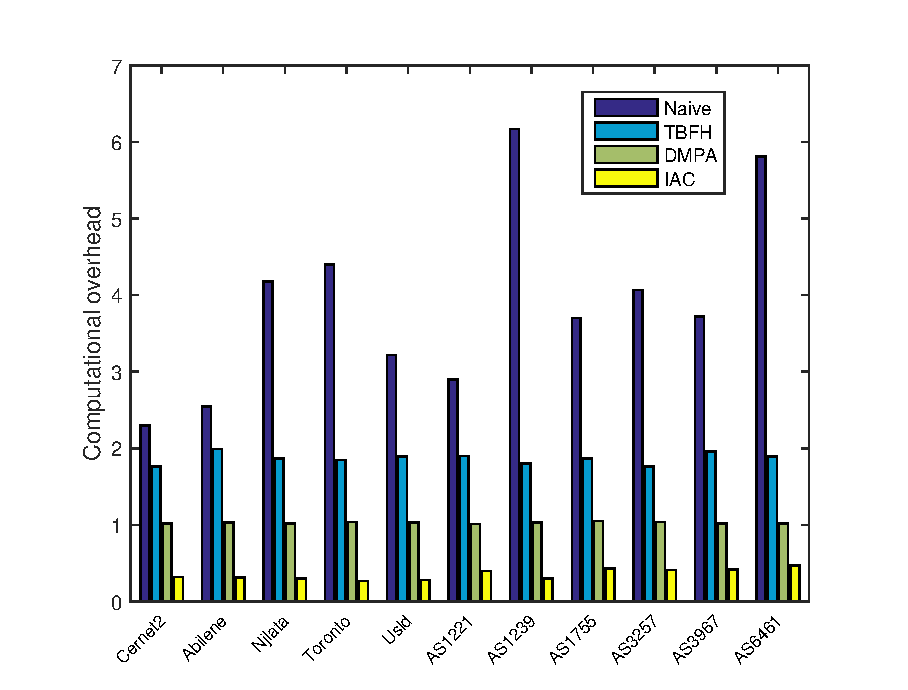
\includegraphics[width=3in]{realcomputationoverhead}
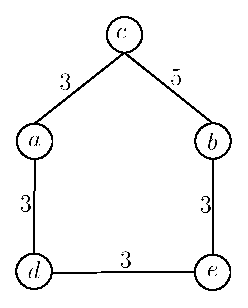
\includegraphics[width=2in]{nettopology}
\caption{network topology}
\label{realandrockettopologytime}
\end{figure}
\begin{figure}[t]
\centering
%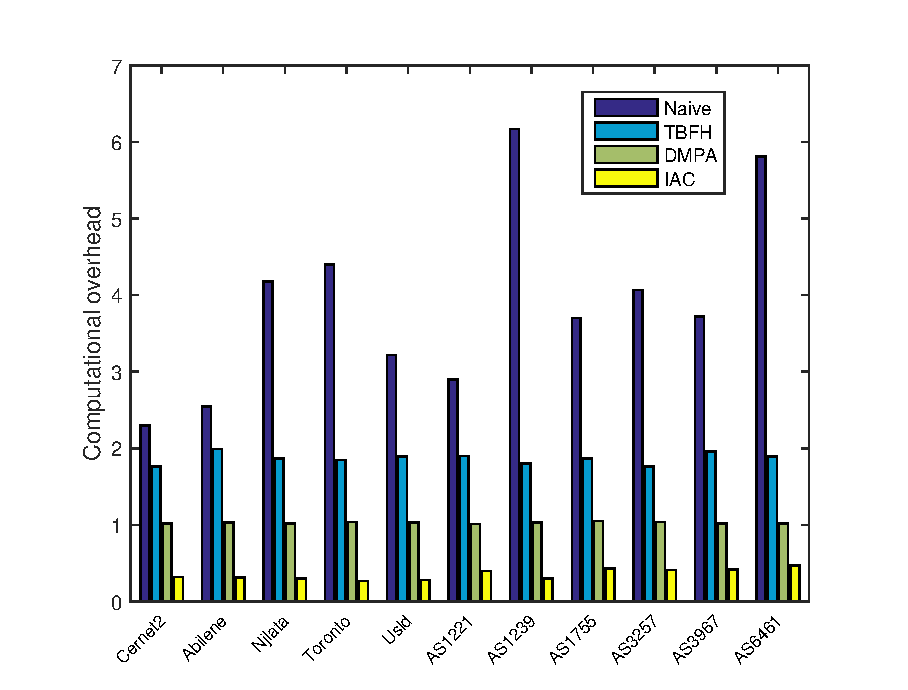
\includegraphics[width=3in]{realcomputationoverhead}
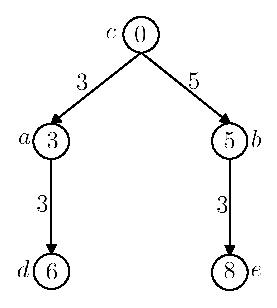
\includegraphics[width=2in]{sptc}
\caption{Shortest path tree rooted at node $c$}
\label{realandrockettopologytime}
\end{figure}
\begin{figure}[t]
\centering
%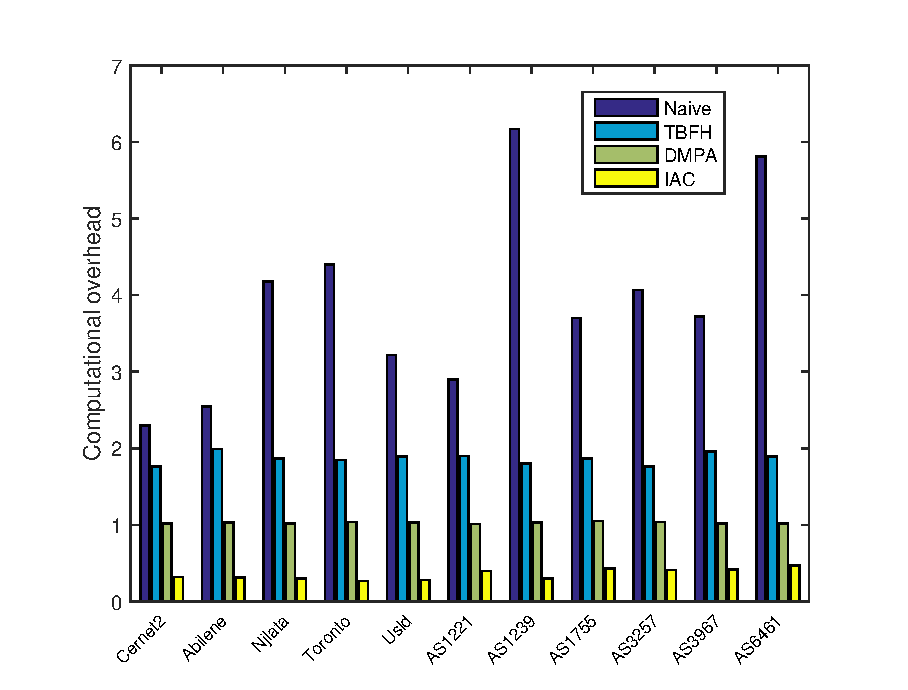
\includegraphics[width=3in]{realcomputationoverhead}
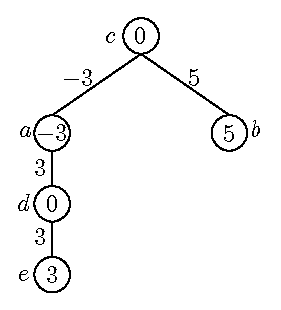
\includegraphics[width=2in]{newsptc}
\caption{New shortest path tree rooted at node $c$}
\label{realandrockettopologytime}
\end{figure}
\fi

\iffalse
\subsection{IAC-NC}
\iffalse
\begin{algorithm}[htb]
\KwIn{Network graph $G=(V,E)$}
\KwIn{$T_c$}
\KwOut{$N_c(v), (\forall v \in V \land v \neq c) $}
%\SetAlgoNoLine
%\SetAlgoNoEnd
\For{$x \in N(c)$}{
\For{$v \in V$}{
 $v.visited \leftarrow false$\;
 $C'_c(v) \leftarrow C_c(v)$\;
}
$c.visited=true$\;
 $weight\leftarrow L(c,x) $\;
 $L(c,x)\leftarrow -L(c,x)$\;

 $\delta\leftarrow weight-L(c,x)$\;
\For{$m\in D(T_c,x)$}
{
$C'_c(m)\leftarrow C'_c(m)-\delta$\;
$m.visited=true$\;
}
\For{$v \in D(T_c,x)$}{
\For {each neighbor $u$ of $v$}{
\If {$u.visited=false$ }
{
$newdist \leftarrow C'_c(v)+L(v,u)$\;
\If {$newdist <C'_c(u)$}{
ENQUEUE$(Q,(u,(v,newdist,\delta))$\;}
}
}
}

\While {$Q$ is not empty}{
$<v,tc> \leftarrow$ EXTRACTMIN(Q)\;

$v.visited\leftarrow true$\;
$C'_c(v)\leftarrow tc$\;

Compute $C_x(v)$ using Theorem \ref{computeneighborcost}\;
\For {each neighbor $u$ of $v$}{
\If {$u.visited=false$ }
{
$newdist \leftarrow C'_c(v)+L(v,u)$\;
\If {$newdist <C'_c(u)$}{
$\delta \leftarrow newdist-C'_c(u)$
ENQUEUE$(Q,(u,(v,newdist,\delta))$\;}
}
}
}
 $L(c,x)\leftarrow weight$\;
}
\For {$d\in V, d \neq c$}{
\For{$x\in N(c)$}
{
 \If {LFA is satisfied}
 {
 Add $x$ to $N_c(d)$\;
 }
}
}

\Return $N_c(v), (\forall v \in V \land v \neq c)$
\caption{IAC-NA}
\label{mnpe}
\end{algorithm}
\fi
Since the execution process of algorithm INC and INC-NA is basically similar, we will not repeat the same part in both of the algorithms.
Below, we will list the differences between the two algorithms. The line 7 in INC-NA is changed into $L(c,x)=-L(c,x)$. The line 22 in INC-NA is changed into Compute $C_x(v)$ using Theorem \ref{computeneighborcost}.
At last lines 29-32 are added to compute LFA next hop set for node $c$.
\fi
%However, for the completeness of the description, we still lists the pseudo code of the algorithm INC-NA.
%
\iffalse
We will elaborate the algorithm in detail in this section.
According to the above discussions, algorithm INC is proposed to compute the backup next-hop set which satisfies the DC rule. The inputs of the INC are the network topology $G=(V,E)$ and $T_{c}$, and the output is the backup next-hop set from node $c$ to all  other nodes in the network.
The INC requires several iterations. In each iteration,
at the beginning, the $visited$ attribute of all nodes except $c$ are set to $false$ (lines 2 $\sim$ 5). We change the weight of the link  $(c,x)$  to $-L(c,x)$, and compute the weight change for $(c,x)$ (lines 6 $\sim$ 8), which is  stored in variable $\delta$. The shortest cost from $c$ to $v$ and the $visited$ attribute of node $v$ are updated accordingly (lines 9 $\sim$ 11).
For $v \in D(T_c,x)$, for each of its unvisited neighbor $u$,
we compute the  new tentative cost  of $u$. The node $u$ will be inserted into
the $Q$ if its new tentative cost is smaller than the old value (lines 12 $\sim$ 17).
An $unvisited$ node $v$ with the lowest tentative cost will be popped out from the priority queue $Q$
by the EXTRACTMIN operation, where node ID is  used as tie breaking.
Then we can compute $C_x(v)$ using Theorem \ref{computeneighborcost}.
It is then added to the tree, marked as $visited$, and used as the $current\ node$ in the iteration,
while its attribute like cost  is also set to
a permanent value (lines $19 \sim 21$).
The corresponding node $x$ is added to the next-hop set $N_{c}(v)$
according to Theorem \ref{lfcbackupnexthop} (line 22).
For each unvisited neighbor $u$ of $v$,
we compute the  new tentative cost  of $u$. The node $u$ will be inserted into
the $Q$ if its new tentative cost is smaller than the old value (lines 23 $\sim$ 27).
At last, we will restore the weight of the link $(c,x)$ (line 28).
The LFA rule is used to calculate the backup next hop set from the node $c$ to all other nodes in the network.
\fi
%\subsection{Theoretical Analysis}
\iffalse
\begin{theorem}\label{mpnecomplexity}
The computational complexity of IAC-NA is less than $O(|E|lg|V|)$ when the queue is implemented as a Heap.
\end{theorem}
The proof for Theorem \ref{mpnecomplexity} is similar with that of Theorem \ref{iaccomplexity}, so we omit it.
\fi


\iffalse
\section{iSPF and LFA}\label{back}
In this section, we will discuss incremental shortest
path first (iSPF) algorithm and LFA, both of which are the foundation of our
work.
\subsection{Incremental Shortest Path First Algorithm}
The OSPF and IS-IS routing protocols which are
widely deployed in today��s Internet calculate a shortest path tree (SPT) from each router to other routers in an autonomous system (AS). Lots of commercial routers have adopted dynamic SPT algorithms which employ the structure of the previously computed SPT rather than recomputed an new SPT from scratch when the network topology changes. The reason is that when network topology changes, the new computed SPT does not differ conspicuously from the old one.

The incremental shortest path first algorithm (iSPF) maintains
a queue $Q$, each element in the queue is
of the form $(n,(p,d,\delta))$ , where $p$ denotes a potential parent
for node $n$, $d$ denotes a potential cost for node  $n$ , and $\delta$ denotes the potential cost change for node  $n$.
The  iSPF \cite{Narv2002New} is carried out as following steps:\\
(1)
Finding all the potentially affected nodes and marking them  \textsl{floating}.\\
(2) Computing the potential new cost, parent and the cost change $\delta$ between
the old cost and the potential new cost for the potentially affected nodes.\\
(3) In each iteration, a node with the smallest $\delta$ (least positive or most negative) is selected, and then a subtree, instead of only
one node, is appended to the new SPT. All of the above nodes are marked  \textsl{anchored}.
\begin{figure*}[t]
        \begin{subfigure}[b]{0.33\textwidth}
                \centering
                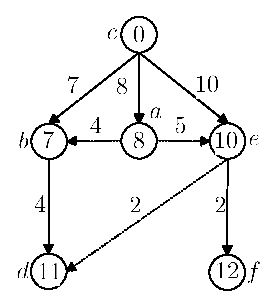
\includegraphics{ispfspt}
                \centering
                \caption{$T_{c}$}
              \label{spttree11}
        \end{subfigure}
        \begin{subfigure}[b]{0.33\textwidth}
                \centering
                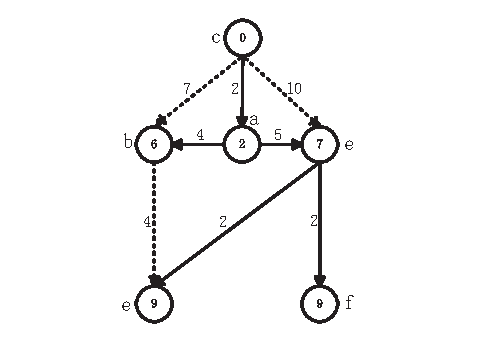
\includegraphics{ispfchange}
                \caption{shortest path tree when the $L(c,a)=2$}
                \label{spttreechange12}
        \end{subfigure}
         \begin{subfigure}[b]{0.33\textwidth}
                \centering
                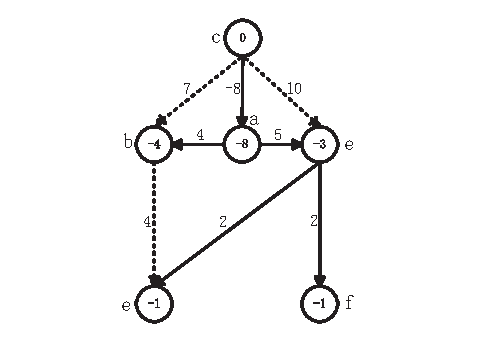
\includegraphics{ispfchange2}
                \caption{$T_{c}^{G_{(c,a)}}$}
                \label{spttreechange13}
        \end{subfigure}
        \caption{An example for explaining iSPF}
        \label{ex}
\end{figure*}
\iffalse
\begin{figure}[t]

\centering
%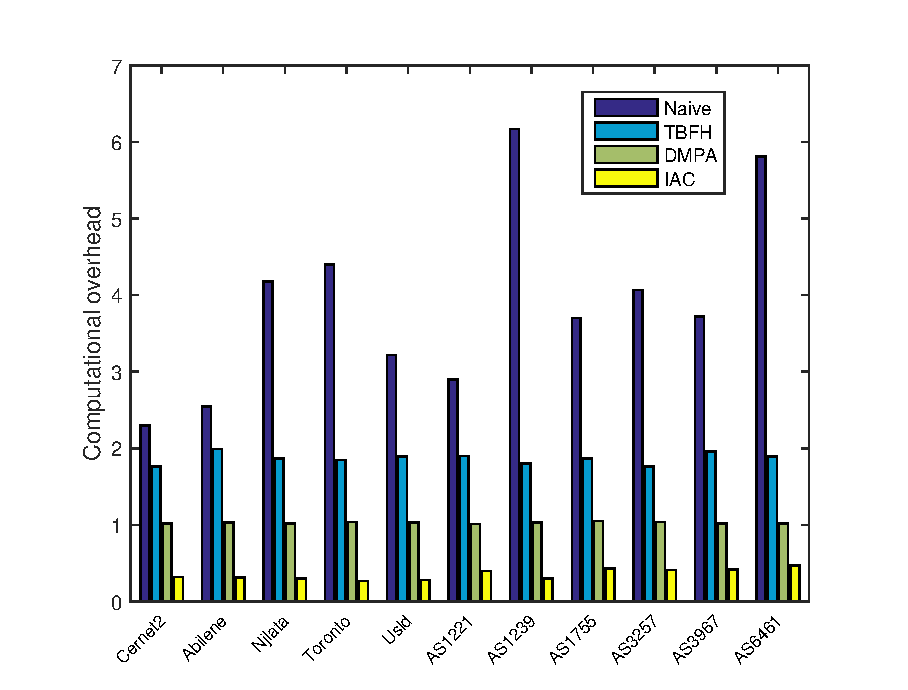
\includegraphics[width=3in]{realcomputationoverhead}
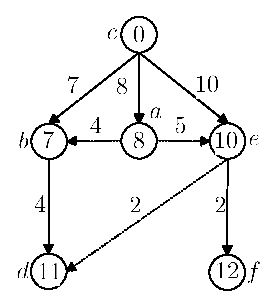
\includegraphics[width=3in]{ispfspt}
\caption{Shortest path tree rooted at $A$ before link change}
\label{ispfsptA}
\end{figure}
\begin{figure}[t]
\centering
%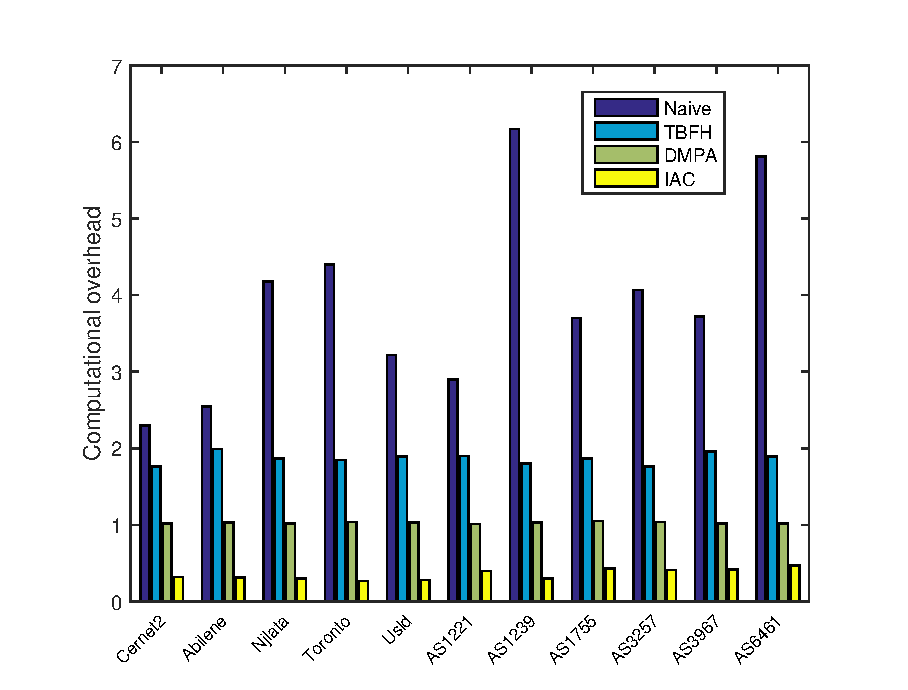
\includegraphics[width=3in]{realcomputationoverhead}
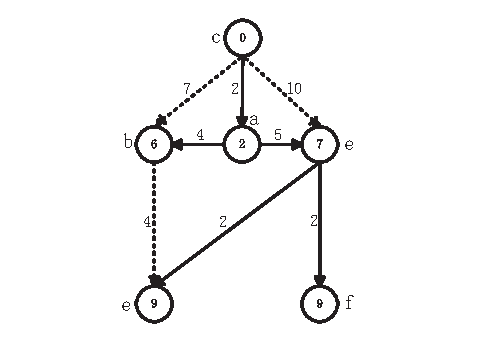
\includegraphics[width=3in]{ispfchange}
\caption{Shortest path tree rooted at $A$ when the weight of $(A,C)$ is changed to 2}
\label{ispfchangeA}
\end{figure}

\begin{figure}[t]
\centering
%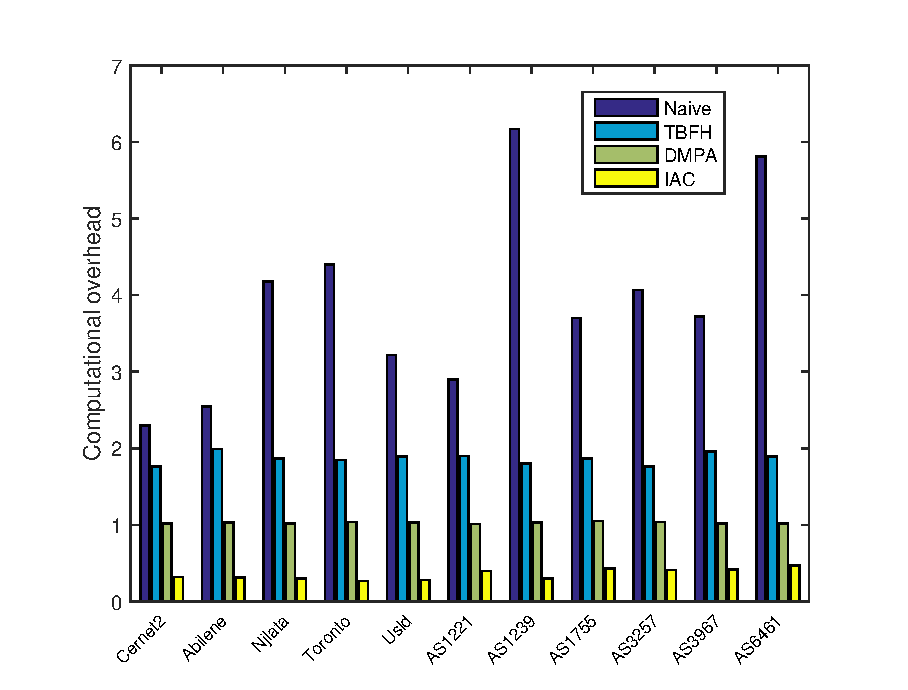
\includegraphics[width=3in]{realcomputationoverhead}
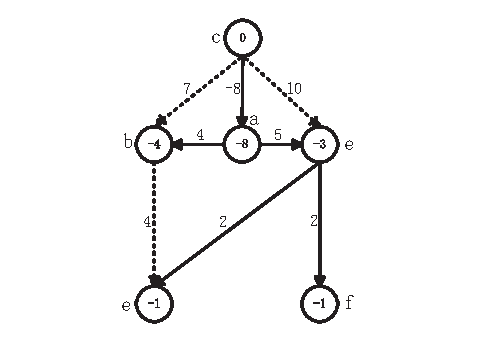
\includegraphics[width=3in]{ispfchange2}
\caption{Shortest path tree rooted at $A$ when the weight of $(A,C)$ is changed to -8}
\label{ispfchangeB}
\end{figure}
\fi

Perhaps the most intuitive way to demonstrate iSPF is through an
example. Consider the network topology depicted in Fig. \ref{spttree11}, which is composed of 6 nodes and 8 links. The letter besides the node is its label.
The solid lines are the links in the shortest path tree which is rooted at node $c$, while the dotted lines are the links  not in the above shortest path tree. The number inside the circle is the shortest cost from node $c$ to that node.

At some point, the weight of the edge $(c,a)$ is changed from 8 to 2.
Nodes except $c$ all affected nodes and are marked as \textsl{floating}.
Only the root node $c$ is marked as \textsl{anchored}. For all the \textsl{floating} nodes,
we check whether they have links to the \textsl{anchored} nodes, and calculate the new cost and the change  in cost. If the change in cost is smaller than 0, the node will be enqueued into the $Q$.
In the first iteration, the $Q$ has only one element with the form of
\{$(a,(c,2,-6))$\}.
In the next iteration, $(a,(c,2,6))$ will be selected and $a$ will be marked as \textsl{anchored}. Since $a$ has an outing edge to $e$ and $b$, the new cost and $\delta$ of $b$ and $e$ is calculated, which gives queue \{$(b,(a,6,-1)),(e,(a,7,-3))$\}. Then $e$ is selected, instead of only marking $e$ as \textsl{anchored}, the original subtree rooted at $e$  is considered together. Therefore the node $f$ is selected and marked as \textsl{anchored} at the same time. Since $e$ has an outing edge to $d$, the new cost and $\delta$ of $d$ is calculated, which gives queue \{$(b,(a,6,-1)),(d,(e,9,-2))$\}. Since node $d$ has the
largest potential shortest cost decrease, node $d$ is marked as \textsl{anchored}.
In the next iteration, node $b$ is selected.
The new shortest path tree is depicted in the
Fig. \ref{spttreechange12}.


Here we will describe a special example, when a single link changes its weight to the opposite number. For example, the weight of the edge $(c,a)$ is changed from 8 to -8. Only the root node $c$ is marked as anchored. For all the floating nodes,
we check whether they have links to the anchored nodes, and calculate the new cost and the change in cost, which gives
queue \{$(a,(c,2,-16))$\}.
In the next iteration, $(a,(c,2,-16))$ will be selected and  $a$ will be marked as anchored. Since $a$ has an outing edge to $e$ and $b$, the new cost and $\delta$ of $e$ and $b$ is calculated, which gives queue \{$(a,(b,-4,-11)),(e,(a,-3,-13))$\}. Then $e$ is selected, instead of only marking $e$ as anchored, the original subtree rooted at $e$  is considered together. Therefore the node $f$ is selected and marked as anchored at the same time. Since $e$ has an outing edge to $d$, the new cost and $\delta$ of $d$ is calculated, which gives queue \{$(a,(b,-4,-11)),(d,(e,-1,-12))$\}. Since node $d$ has the
largest potential shortest cost decrease, node $d$ is marked as anchored.
In the next iteration, node $b$ is selected.
The new shortest path tree is given in the
Fig. \ref{spttreechange13}.
\subsection{Some properties of the iSPF}
\fi
